% Options for packages loaded elsewhere
\PassOptionsToPackage{unicode}{hyperref}
\PassOptionsToPackage{hyphens}{url}
\PassOptionsToPackage{dvipsnames,svgnames,x11names}{xcolor}
%
\documentclass[
  a4paper,
  DIV=11,
  numbers=noendperiod]{scrartcl}

\usepackage{amsmath,amssymb}
\usepackage{iftex}
\ifPDFTeX
  \usepackage[T1]{fontenc}
  \usepackage[utf8]{inputenc}
  \usepackage{textcomp} % provide euro and other symbols
\else % if luatex or xetex
  \usepackage{unicode-math}
  \defaultfontfeatures{Scale=MatchLowercase}
  \defaultfontfeatures[\rmfamily]{Ligatures=TeX,Scale=1}
\fi
\usepackage{lmodern}
\ifPDFTeX\else  
    % xetex/luatex font selection
    \setmainfont[]{Spectral}
    \setsansfont[]{Roboto Flex}
    \setmonofont[]{InputMonoCondensed}
\fi
% Use upquote if available, for straight quotes in verbatim environments
\IfFileExists{upquote.sty}{\usepackage{upquote}}{}
\IfFileExists{microtype.sty}{% use microtype if available
  \usepackage[]{microtype}
  \UseMicrotypeSet[protrusion]{basicmath} % disable protrusion for tt fonts
}{}
\makeatletter
\@ifundefined{KOMAClassName}{% if non-KOMA class
  \IfFileExists{parskip.sty}{%
    \usepackage{parskip}
  }{% else
    \setlength{\parindent}{0pt}
    \setlength{\parskip}{6pt plus 2pt minus 1pt}}
}{% if KOMA class
  \KOMAoptions{parskip=half}}
\makeatother
\usepackage{xcolor}
\usepackage[top=25mm,left=40mm,right=30mm,bottom=25mm,heightrounded]{geometry}
\setlength{\emergencystretch}{3em} % prevent overfull lines
\setcounter{secnumdepth}{-\maxdimen} % remove section numbering
% Make \paragraph and \subparagraph free-standing
\makeatletter
\ifx\paragraph\undefined\else
  \let\oldparagraph\paragraph
  \renewcommand{\paragraph}{
    \@ifstar
      \xxxParagraphStar
      \xxxParagraphNoStar
  }
  \newcommand{\xxxParagraphStar}[1]{\oldparagraph*{#1}\mbox{}}
  \newcommand{\xxxParagraphNoStar}[1]{\oldparagraph{#1}\mbox{}}
\fi
\ifx\subparagraph\undefined\else
  \let\oldsubparagraph\subparagraph
  \renewcommand{\subparagraph}{
    \@ifstar
      \xxxSubParagraphStar
      \xxxSubParagraphNoStar
  }
  \newcommand{\xxxSubParagraphStar}[1]{\oldsubparagraph*{#1}\mbox{}}
  \newcommand{\xxxSubParagraphNoStar}[1]{\oldsubparagraph{#1}\mbox{}}
\fi
\makeatother


\providecommand{\tightlist}{%
  \setlength{\itemsep}{0pt}\setlength{\parskip}{0pt}}\usepackage{longtable,booktabs,array}
\usepackage{calc} % for calculating minipage widths
% Correct order of tables after \paragraph or \subparagraph
\usepackage{etoolbox}
\makeatletter
\patchcmd\longtable{\par}{\if@noskipsec\mbox{}\fi\par}{}{}
\makeatother
% Allow footnotes in longtable head/foot
\IfFileExists{footnotehyper.sty}{\usepackage{footnotehyper}}{\usepackage{footnote}}
\makesavenoteenv{longtable}
\usepackage{graphicx}
\makeatletter
\def\maxwidth{\ifdim\Gin@nat@width>\linewidth\linewidth\else\Gin@nat@width\fi}
\def\maxheight{\ifdim\Gin@nat@height>\textheight\textheight\else\Gin@nat@height\fi}
\makeatother
% Scale images if necessary, so that they will not overflow the page
% margins by default, and it is still possible to overwrite the defaults
% using explicit options in \includegraphics[width, height, ...]{}
\setkeys{Gin}{width=\maxwidth,height=\maxheight,keepaspectratio}
% Set default figure placement to htbp
\makeatletter
\def\fps@figure{htbp}
\makeatother
% definitions for citeproc citations
\NewDocumentCommand\citeproctext{}{}
\NewDocumentCommand\citeproc{mm}{%
  \begingroup\def\citeproctext{#2}\cite{#1}\endgroup}
\makeatletter
 % allow citations to break across lines
 \let\@cite@ofmt\@firstofone
 % avoid brackets around text for \cite:
 \def\@biblabel#1{}
 \def\@cite#1#2{{#1\if@tempswa , #2\fi}}
\makeatother
\newlength{\cslhangindent}
\setlength{\cslhangindent}{1.5em}
\newlength{\csllabelwidth}
\setlength{\csllabelwidth}{3em}
\newenvironment{CSLReferences}[2] % #1 hanging-indent, #2 entry-spacing
 {\begin{list}{}{%
  \setlength{\itemindent}{0pt}
  \setlength{\leftmargin}{0pt}
  \setlength{\parsep}{0pt}
  % turn on hanging indent if param 1 is 1
  \ifodd #1
   \setlength{\leftmargin}{\cslhangindent}
   \setlength{\itemindent}{-1\cslhangindent}
  \fi
  % set entry spacing
  \setlength{\itemsep}{#2\baselineskip}}}
 {\end{list}}
\usepackage{calc}
\newcommand{\CSLBlock}[1]{\hfill\break\parbox[t]{\linewidth}{\strut\ignorespaces#1\strut}}
\newcommand{\CSLLeftMargin}[1]{\parbox[t]{\csllabelwidth}{\strut#1\strut}}
\newcommand{\CSLRightInline}[1]{\parbox[t]{\linewidth - \csllabelwidth}{\strut#1\strut}}
\newcommand{\CSLIndent}[1]{\hspace{\cslhangindent}#1}

\addtokomafont{disposition}{\rmfamily}
\KOMAoption{captions}{tableheading}
\makeatletter
\@ifpackageloaded{caption}{}{\usepackage{caption}}
\AtBeginDocument{%
\ifdefined\contentsname
  \renewcommand*\contentsname{Table of contents}
\else
  \newcommand\contentsname{Table of contents}
\fi
\ifdefined\listfigurename
  \renewcommand*\listfigurename{List of Figures}
\else
  \newcommand\listfigurename{List of Figures}
\fi
\ifdefined\listtablename
  \renewcommand*\listtablename{List of Tables}
\else
  \newcommand\listtablename{List of Tables}
\fi
\ifdefined\figurename
  \renewcommand*\figurename{Figure}
\else
  \newcommand\figurename{Figure}
\fi
\ifdefined\tablename
  \renewcommand*\tablename{Table}
\else
  \newcommand\tablename{Table}
\fi
}
\@ifpackageloaded{float}{}{\usepackage{float}}
\floatstyle{ruled}
\@ifundefined{c@chapter}{\newfloat{codelisting}{h}{lop}}{\newfloat{codelisting}{h}{lop}[chapter]}
\floatname{codelisting}{Listing}
\newcommand*\listoflistings{\listof{codelisting}{List of Listings}}
\makeatother
\makeatletter
\makeatother
\makeatletter
\@ifpackageloaded{caption}{}{\usepackage{caption}}
\@ifpackageloaded{subcaption}{}{\usepackage{subcaption}}
\makeatother

\ifLuaTeX
  \usepackage{selnolig}  % disable illegal ligatures
\fi
\usepackage{bookmark}

\IfFileExists{xurl.sty}{\usepackage{xurl}}{} % add URL line breaks if available
\urlstyle{same} % disable monospaced font for URLs
\hypersetup{
  pdftitle={Group Name's Group Project},
  colorlinks=true,
  linkcolor={blue},
  filecolor={Maroon},
  citecolor={Blue},
  urlcolor={Blue},
  pdfcreator={LaTeX via pandoc}}


\title{Group Name's Group Project}
\author{}
\date{}

\begin{document}
\maketitle


\subsection*{Declaration of Authorship}\label{declaration-of-authorship}

We, {[}insert your group's names{]}, pledge our honour that the work
presented in this assessment is our own. Where information has been
derived from other sources, we confirm that this has been indicated in
the work. Where a Large Language Model such as ChatGPT has been used we
confirm that we have made its contribution to the final submission
clear.

Date:

Student Numbers:

\subsection{Brief Group Reflection}\label{brief-group-reflection}

\begin{longtable}[]{@{}ll@{}}
\toprule\noalign{}
What Went Well & What Was Challenging \\
\midrule\noalign{}
\endhead
\bottomrule\noalign{}
\endlastfoot
A & B \\
C & D \\
\end{longtable}

\subsection{Priorities for Feedback}\label{priorities-for-feedback}

Are there any areas on which you would appreciate more detailed feedback
if we're able to offer it?

\newpage{}

\section{Response to Questions}\label{response-to-questions}

See the raw file for examples of how to hide computational output as
there is code hidden here.

\subsection{1. Who collected the InsideAirbnb
data?}\label{who-collected-the-insideairbnb-data}

( 2 points; Answer due Week 7 )

An inline citation example: As discussed on {`Inside airbnb'} (n.d.),
there are many\ldots{}

A parenthetical citation example: There are many ways to research Airbnb
(see, for example, {`Inside airbnb'}, n.d.)\ldots{}

\subsection{2. Why did they collect the InsideAirbnb
data?}\label{why-did-they-collect-the-insideairbnb-data}

( 4 points; Answer due Week 7 )

One of way to embed output in the text looks like this: after cleaning,
we were left with 85,127 rows of data.

This way is also supposed to work
(\texttt{\{python\}\ f"\{df.shape{[}0{]}:,\}"}) but I've found it less
reliable.

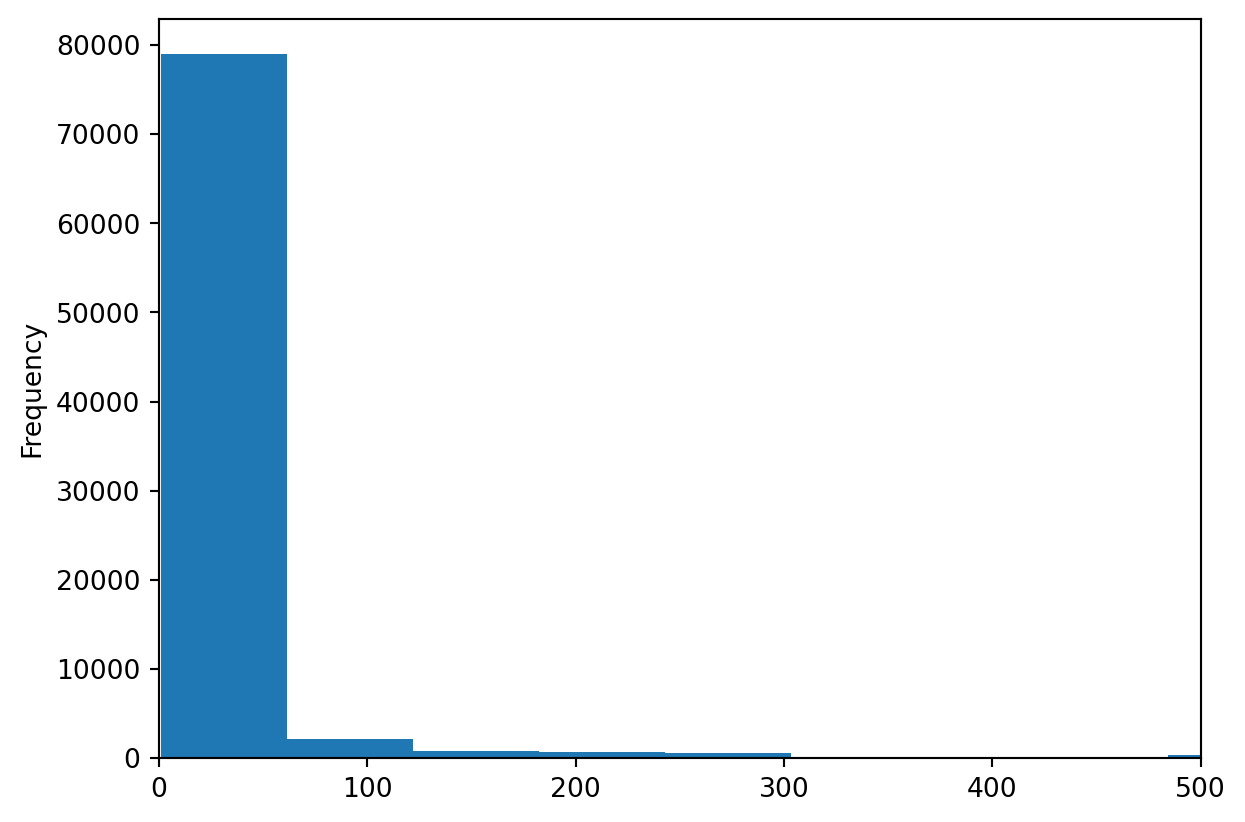
\includegraphics{Group_Work_files/figure-pdf/cell-5-output-1.pdf}

\subsection{3. How did they collect it?}\label{how-did-they-collect-it}

( 5 points; Answer due Week 8 )

\subsection{4. How does the method of collection (Q3) impact the
completeness and/or accuracy of the InsideAirbnb data? How well does it
represent the process it seeks to study, and what wider issues does this
raise?}\label{how-does-the-method-of-collection-q3-impact-the-completeness-andor-accuracy-of-the-insideairbnb-data-how-well-does-it-represent-the-process-it-seeks-to-study-and-what-wider-issues-does-this-raise}

( 11 points; Answer due Week 9 )

\subsection{5. What ethical considerations does the use of the
InsideAirbnb data
raise?}\label{what-ethical-considerations-does-the-use-of-the-insideairbnb-data-raise}

( 18 points; Answer due \textbf{?var:assess.group-date} )

\subsection{\texorpdfstring{6. With reference to the InsideAirbnb data
(\emph{i.e.} using numbers, figures, maps, and descriptive statistics),
what does an analysis of Hosts and the types of properties that they
list suggest about the nature of Airbnb lettings in
London?}{6. With reference to the InsideAirbnb data (i.e. using numbers, figures, maps, and descriptive statistics), what does an analysis of Hosts and the types of properties that they list suggest about the nature of Airbnb lettings in London?}}\label{with-reference-to-the-insideairbnb-data-i.e.-using-numbers-figures-maps-and-descriptive-statistics-what-does-an-analysis-of-hosts-and-the-types-of-properties-that-they-list-suggest-about-the-nature-of-airbnb-lettings-in-london}

( 15 points; Answer due \textbf{?var:assess.group-date} )

\subsection{\texorpdfstring{7. Drawing on your previous answers, and
supporting your response with evidence (\emph{e.g.} figures, maps,
EDA/ESDA, and simple statistical analysis/models drawing on experience
from, e.g., CASA0007), how \emph{could} the InsideAirbnb data set be
used to inform the regulation of Short-Term Lets (STL) in
London?}{7. Drawing on your previous answers, and supporting your response with evidence (e.g. figures, maps, EDA/ESDA, and simple statistical analysis/models drawing on experience from, e.g., CASA0007), how could the InsideAirbnb data set be used to inform the regulation of Short-Term Lets (STL) in London?}}\label{drawing-on-your-previous-answers-and-supporting-your-response-with-evidence-e.g.-figures-maps-edaesda-and-simple-statistical-analysismodels-drawing-on-experience-from-e.g.-casa0007-how-could-the-insideairbnb-data-set-be-used-to-inform-the-regulation-of-short-term-lets-stl-in-london}

( 45 points; Answer due \textbf{?var:assess.group-date} )

\subsection{Sustainable Authorship
Tools}\label{sustainable-authorship-tools}

Using the Terminal in Docker, you compile the Quarto report using
\texttt{quarto\ render\ \textless{}group\_submission\_file\textgreater{}.qmd}.

Your QMD file should automatically download your BibTeX and CLS files
and any other required files. If this is done right after library
loading then the entire report should output successfully.

Written in Markdown and generated from
\href{https://quarto.org/}{Quarto}. Fonts used:
\href{https://fonts.google.com/specimen/Spectral}{Spectral} (mainfont),
\href{https://fonts.google.com/specimen/Roboto}{Roboto} ({sansfont}) and
\href{https://fonts.google.com/specimen/JetBrains\%20Mono}{JetBrains
Mono} (\texttt{monofont}).

\subsection*{References}\label{references}
\addcontentsline{toc}{subsection}{References}

\phantomsection\label{refs}
\begin{CSLReferences}{0}{1}
\bibitem[\citeproctext]{ref-insideairbnb}
{`Inside airbnb'} (n.d.). Available at: \url{http://insideairbnb.com}.

\end{CSLReferences}




\end{document}
